\documentclass{beamer}
\usepackage[utf8]{inputenc}
\usepackage[backend=biber, style=authoryear]{biblatex}
\addbibresource{bib.bib}
\usepackage{adjustbox}
\usepackage{booktabs}
\usepackage{siunitx}
\usepackage{amsmath}
\usepackage{amssymb}
\usepackage{amsthm}
\usepackage{yhmath}
\newcolumntype{d}{S[
	input-open-uncertainty=,
	input-close-uncertainty=,
	parse-numbers = false,
	table-align-text-pre=false,
	table-align-text-post=false
	]}

\usepackage{mathtext} 				% русские буквы в формулах
\usepackage[T2A]{fontenc}			% кодировка
\usepackage[utf8]{inputenc}			% кодировка исходного текста
\usepackage[english]{babel}	% локализация и переносы

\usetheme{boxes}
\usecolortheme{default}

\setbeamertemplate{caption}{\insertcaption}
\setbeamertemplate{enumerate items}[circle]
\setbeamertemplate{itemize items}[circle]

% Title page details
\title[Social support in victim crime reporting]{\textquoteleft You should call the police\textquoteright:\\Social support in crime victim reporting}
%\subtitle{Quick-start guide}
\author[Bondarkov]{Sergey Bondarkov}
\institute[IRL]{Institute for the Rule of Law, EUSPb}
\date{\today}

\newcommand\Wider[2][3em]{%
	\makebox[\linewidth][c]{%
		\begin{minipage}{\dimexpr\textwidth+#1\relax}
			\raggedright#2
		\end{minipage}%
	}%
}

\begin{document}

% Title page
\begin{frame}
	\titlepage
\end{frame}

% Presentation outline
\begin{frame}{Outline}
	\tableofcontents[hideallsubsections]
\end{frame}

% ==================================================================

\section{This talk in a nutshell}
\begin{frame}{This talk in a nutshell}
	\begin{itemize}
		\item Victims of crime not always notify the police
		\item This distorts the enforcer's view of crime and, in some scenarios, precludes victims from receiving help
		\item One theoretical factor of reporting that is understudied is\\ \textbf{the ability to talk the incident through\\with friends or family}
		\item I attempt to identify the factor's effect using data from\\RCVS 2024
		\item Regression results back up expectations, but a plausible backdoor remains
		\item IV to the rescue, but the instrument is too weak  
	\end{itemize}	
\end{frame}

% ==================================================================

\section{The problem}
%\begin{frame}{Problem illustration: Russian case}
%	Victimization estimates: RCVS vs Crimestat 
%\end{frame}

\begin{frame}{Why is non-reporting a problem?}
	\begin{itemize}
		\item Non-reporting distorts the enforcer's view of crime rates and structure which precludes optimal resource allocation for crime prevention.
		\item In a broader sense, under-reporting distorts understanding of how crime impacts individuals, communities and neighborhoods. This has implications both for administration and legislation.
		\item In some situations, e.g. intimate partner violence, early intervention from authority can prevent progressively heavier damage -- this can not happen if the police is not notified.
	\end{itemize}
\end{frame}

% ==================================================================

\section{Theoretical models of crime reporting}
\begin{frame}{Theoretical models of crime reporting}

	\begin{itemize}
		\item Macrosociological: \textcite{black1976behavior} posited that mobilization of law can be explained by stratification, morphology, culture, organization, and social control.
		\item Rational choice: The main determinants of decision to notify the police relate to gravity of incident and perceived costs and benefits of reporting \parencite{gottfredson1979study, skogan1984reporting, tarling2010reporting}.
		\begin{itemize}
			\item This view has been criticized on the grounds that a victim never has full information and is usually in a condition that compromises his or hers ability for calculation of costs and benefits \parencite{gottfredson1987decision}.
		\end{itemize}
		\item Attitudes: This view focuses on perception of police legitimacy and ability, as well as on gender roles and victim blaming \parencite{tyler2003procedural,orcutt1988sex}.
		\item Social influence: decision making is a complex process which is affected by a victim's social context \parencite{greenberg2012after}.
	\end{itemize}
\end{frame}

\begin{frame}{Greenberg and Ruback's victim decision making model}
	\Wider[4em]{
		\begin{figure}
			\includegraphics[width=\textwidth]{../../output/figures/decision_model}
		\end{figure}
	}
	\\
	\vspace{3mm}
	\small Adapted from \textcite{greenberg2012after}
\end{frame}

% ==================================================================

\section{Data}
\begin{frame}{Data: RCVS}
	Russian Crime Victimization Survey (RCVS) \parencite{sereb2022dynamics}
	\begin{itemize}
		\item a regular and nationally representative victimization survey,
		\item targets citizens 18+ years old,
		\item three waves so far: 2018, 2021, 2024,
		\item performed as computer assisted telephone interview (CATI) using a randomly generated set of telephone numbers (RDD),
%		\item each wave proceeds until 3\ 000 self-defined victims are reached,
		\item includes calibration weights obtained via raking procedure.
	\end{itemize}
\end{frame}

\begin{frame}{Data: 2024 victimization}
	\begin{itemize}
		\item The 2024 survey interviewed 11\ 323 people, with response rate at 0.15--0.91\%.
		\item 2\ 685 respondents said they had been victimized in some way in the past year.
		\item Only 44\% of them notified the police.		
	\end{itemize}
\vspace{10mm}

\Wider[2em]{
	\begin{adjustbox}{width=\textwidth}
		\begin{tabular}[t]{llrrrrr}
			\toprule
			Gender & Reported & Cybercrime & Trad fraud & Theft & Assault & Robbery\\
			\midrule
			Female & 0 & 169 & 2 & 80 & 36 & 4\\
			& 1 & 198 & 10 & 127 & 64 & 17\\
			Male & 0 & 184 & 6 & 85 & 91 & 27\\
			& 1 & 184 & 17 & 134 & 94 & 38\\
			\bottomrule
		\end{tabular}
	\end{adjustbox}
}
\end{frame}

\begin{frame}{Raw conditional means on 2024 data}
	\includegraphics[width=\textwidth]{../../output/figures/raw_means_2024}
\end{frame}

% ==================================================================

\section{Modeling}
\begin{frame}{Identification strategy: Model}
	\begin{figure}
		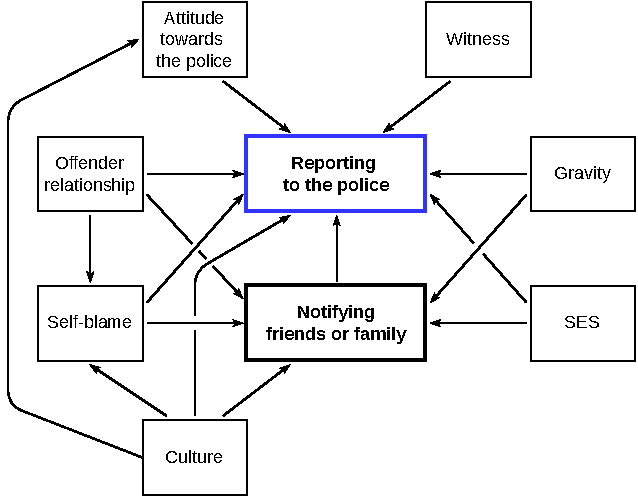
\includegraphics[width=0.9\textwidth]{figures/causal_diagram_1}
	\end{figure}
\end{frame}

\begin{frame}{Identification strategy: Logistic regression}
	\label{eq1}
	\vspace{-7mm}
\begin{equation}
	\begin{aligned}
		P(Reported_i | ToldSomeone = ToldSomeone_i, X_j = x_{ij}) =\\
		\sigma(\beta_0 + \beta_1 ToldSomeone_i + \sum_{1}^{j}\beta_j X_{ij})
	\end{aligned}
\end{equation}
	where
	\begin{itemize}
		\item $Reported$ is unity when a victim notified the police and zero otherwise,
		\item $ToldSomeone$ indicates talking with friends or family about the incident,
		\item and $X$ is a set of $j$ controls which includes measures of financial and emotional damage, reported self-blame, victim's SES, attitude towards police, settlement size type and federal district.\\
	\end{itemize}
	
	In case of violent crimes $X$ also includes level of physical damage, incident features, and type of offender-victim relationship.\\

	\hyperlink{variables}{\beamergotobutton{List of all variables}}
\end{frame}

\begin{frame}{Logistic regression result (abridged)}
\vspace{-.5cm}
		\begin{adjustbox}{width=\textwidth}
	\begin{tabular}{lccccc}
		\toprule
		& Theft & Cybercrime & All property & Assault & All violent\\
		\multicolumn{6}{l}{Dep. var.: Victim notified the police }\\
		\midrule
		\textit{Social factors} & & & & & \\
		Told someone: Yes & \num{1.046} (\num{0.565}) & \num{1.714} (\num{0.465})+ & \num{1.625} (\num{0.473}) & \num{13.057} (\num{9.309})** & \num{12.307} (\num{8.365})**\\
		Self-blame: Yes & \num{0.674} (\num{0.180}) & \num{0.671} (\num{0.150}) & \num{0.621} (\num{0.096})* & \num{0.667} (\num{0.320}) & \num{0.587} (\num{0.278})\\
		Has partner: Yes & \num{0.915} (\num{0.221}) & \num{0.929} (\num{0.166}) & \num{0.946} (\num{0.094}) & \num{1.076} (\num{0.460}) & \num{1.133} (\num{0.352})\\
		Offender relationship & & & & & \\
		\hspace{3mm}Acquaintance or colleague &  &  &  & \num{5.012} (\num{2.984})* & \num{4.833} (\num{2.659})*\\
		\hspace{3mm}Neighbour &  &  &  & \num{7.070} (\num{4.861})* & \num{6.815} (\num{3.067})**\\
		\hspace{3mm}Spouse, partner, relative, friend &  &  &  & \num{1.378} (\num{0.711}) & \num{1.727} (\num{0.834})\\
		\midrule
		\textit{Perceived harm} & & & & & \\
		Financial & & & & & \\
		\hspace{3mm}(1, 10]   thnd rub. & \num{0.962} (\num{0.347}) & \num{2.014} (\num{0.930}) & \num{1.487} (\num{0.583}) & \num{2.484} (\num{1.793}) & \num{2.121} (\num{1.535})\\
		\hspace{3mm}(10, 50]  thnd rub. & \num{2.389} (\num{0.938})+ & \num{3.351} (\num{1.153})** & \num{2.692} (\num{0.795})** & \num{1.347} (\num{1.155}) & \num{2.114} (\num{1.187})\\
		\hspace{3mm}(50, Inf] thnd rub. & \num{3.908} (\num{1.258})** & \num{8.962} (\num{2.664})*** & \num{5.868} (\num{1.588})*** & \num{2.195} (\num{2.144}) & \num{2.642} (\num{1.408})+\\
		Physical & & & & & \\
		\hspace{3mm}Light &  &  &  & \num{0.868} (\num{0.546}) & \num{0.901} (\num{0.406})\\
		\hspace{3mm}Heavy &  &  &  & \num{2.544} (\num{1.732}) & \num{2.472} (\num{1.267})\\
		Emotional & & & & & \\
		\hspace{3mm}Medium & \num{2.386} (\num{1.040})+ & \num{1.075} (\num{0.313}) & \num{1.280} (\num{0.354}) & \num{0.338} (\num{0.245}) & \num{0.375} (\num{0.263})\\
		\hspace{3mm}Heavy & \num{3.499} (\num{1.435})* & \num{2.261} (\num{0.736})* & \num{2.443} (\num{0.621})** & \num{0.813} (\num{0.403}) & \num{1.053} (\num{0.519})\\
		\midrule
		Num. obs. & \num{405} & \num{703} & \num{1143} & \num{260} & \num{304}\\
		Pseudo $R^{2}$ Within & \num{0.135} & \num{0.136}  & \num{0.120} & \num{0.264} & \num{0.272}\\
		RMSE & \num{0.44} & \num{0.45} & \num{0.45} & \num{0.41} & \num{0.41}\\
		Std.Errors & Fed. district & Fed. district & Fed. district & Fed. district & Fed. district\\
		Fixed effects: Fed. district & X & X & X & X & X\\
		\bottomrule
		\vspace{-3mm}\\
		\multicolumn{6}{l}{$+\ p < 0.1$, * $p < 0.05$, ** $p < 0.01$, *** $p < 0.001$}
	\end{tabular}
\end{adjustbox}
\vspace{-.3cm}
\small Coefficients are exponentiated. Only variables of interest are shown.
\end{frame}

\begin{frame}{Avg. predicted prob. of reporting a violent victimization}
	\Wider[3.5em]{
	\begin{figure}
		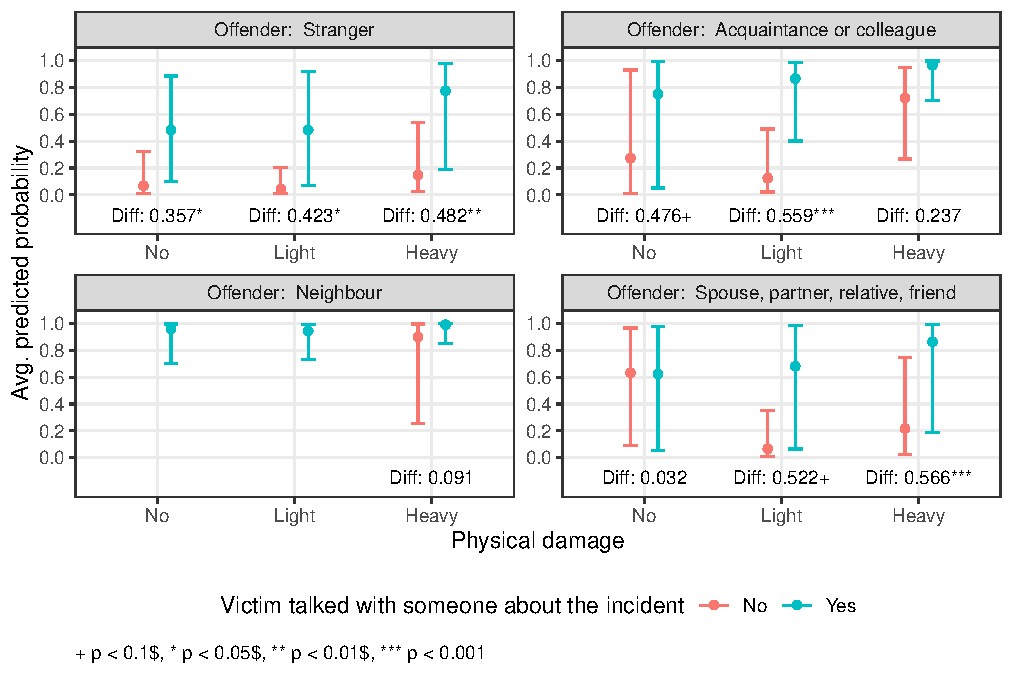
\includegraphics[width=\textwidth]{figures/avg_predicted_probs_grouped}
	\end{figure}
	}
\end{frame}

% ==================================================================
\section{Robustness test}
\begin{frame}{Identification strategy: the plausible backdoor}
	\begin{figure}
		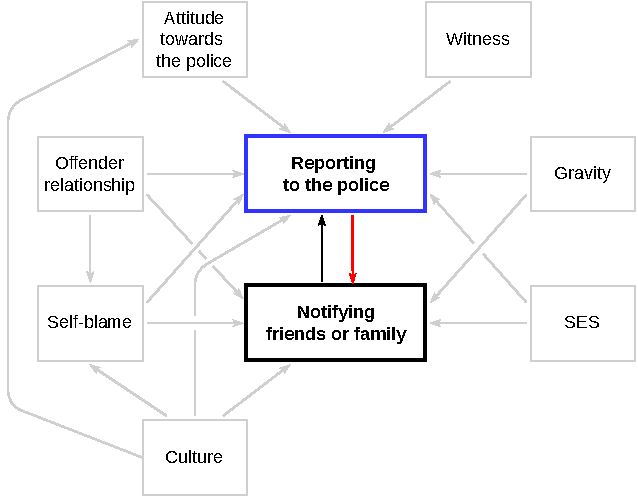
\includegraphics[width=\textheight]{figures/causal_diagram_2}
	\end{figure}
\end{frame}

\begin{frame}{Robustness test: IV regression with 2SLS}
	\begin{figure}
		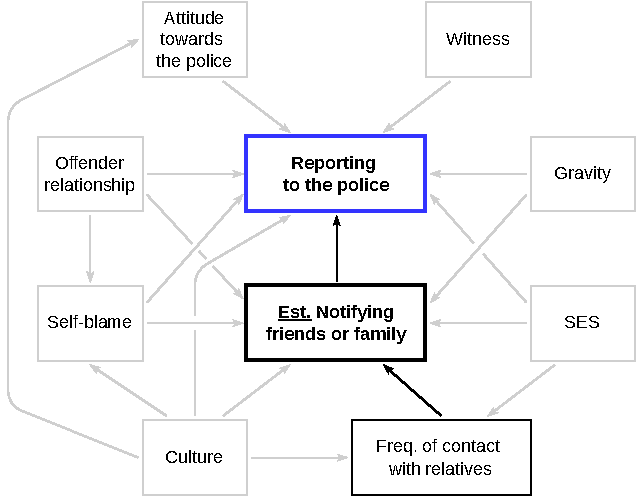
\includegraphics[width=\textheight]{figures/causal_diagram_3}
	\end{figure}
\end{frame}

\begin{frame}{Robustness test: IV regression with 2SLS}
	I assume that frequency of contact with relatives ($ContactRelativesFreq$)
	\begin{itemize}
		\item can explain some variation in $ToldSomeone$,
		\item can not have direct effect on $Reported$,
	\end{itemize}
	\vspace{1mm}
	and therefore may be a suitable instrument in a two-stage least squares (2SLS) regression.\\
	\vspace{3mm}
	First stage:
	\begin{equation}
		ToldSomeone_i = \gamma_0 + \gamma_1 ContactRelativesFreq_i + \gamma_j \sum_{1}^{j}X_{ij} + \upsilon_i
	\end{equation}
	Second stage:
	\begin{equation}
		Reported_i = \beta_0 + \beta_1 \widehat{ToldSomeone_i} + \beta_j \sum_{1}^{j}X_{ij} + \epsilon_i
	\end{equation}
\end{frame}

\begin{frame}{Robustness test: Results}
	\Wider[4em]{
\begin{adjustbox}{width=\textwidth}
	\begin{tabular}[t]{lccccc}
		\toprule
		& Theft & Cybercrime & All property & Assault & All violent\\
		\midrule
		$\widehat{ToldSomeone}$: Yes & \num{-0.732} (\num{0.837}) & \num{0.202} (\num{1.710}) & \num{-0.842} (\num{0.720}) & \num{0.113} (\num{0.311}) & \num{0.130} (\num{0.348})\\
		\midrule
		Num.Obs. & \num{405} & \num{703} & \num{1143} & \num{260} & \num{304}\\
		1st stage F-statistic & 4.296 ($p$:0.014) & 0.453 ($p$:0.635) & 1.928 ($p$:0.146) & 6.587 ($p$:0.002) & 6.389 ($p$:0.002)\\
		R2 Within & \num{-0.028} & \num{0.165} & \num{-0.293} & \num{0.305} & \num{0.308}\\
		RMSE & \num{0.49} & \num{0.45} & \num{0.56} & \num{0.42} & \num{0.41}\\
		Std.Errors & by: Fed. district & by: Fed. district  & by: Fed. district  & by: Fed. district  & by: Fed. district \\
		FE: Fed. district  & X & X & X & X & X\\
		\bottomrule
		\vspace{-3mm}\\
		\multicolumn{6}{l}{$+\ p < 0.1$, * $p < 0.05$, ** $p < 0.01$, *** $p < 0.001$}
	\end{tabular}
\end{adjustbox}}
\\
\vspace{5mm}
\centering
Alas, the instrument proved to be too weak.
\end{frame}

%\begin{frame}{Alas, the instrument is too weak}
%	Table
%\end{frame}

% ==================================================================
\section{Conclusion}
\begin{frame}{Conclusion}
\begin{itemize}
	\item Discussion of victimization with friends or family is the strongest predictor of reporting violent crime to the police --- after controlling for gravity of crime and other possible confounders.
	\item The effect is especially pronounced when offender is closely related to the victim.
	\item However, identification of the effect may be compromised: it is plausible that the effect is driven by victims who \textit{first} notified the police and \textit{then} told someone about the whole thing.
	\item I attempted to rule out endogeneity using frequency of contact with relatives as an instrument for probability of turning to them in case of victimization, but to no avail.
	\item Possible paths to defend the effect: stronger instrument, more data, changes to questionary, \textbf{your suggestions}. 
\end{itemize}
\end{frame}

\begin{frame}{List of all variables \hyperlink{eq1}{\beamergotobutton{Back}}}
\label{variables}

\Wider[2em]{
\scriptsize
\begin{columns}
	\begin{column}{0.5\textwidth}
	Crime gravity
	\begin{itemize}
		\item Financial damage level
		\item Physical damage level
		\item Emotional damage level
	\end{itemize}
	Incident features
	\begin{itemize}
		\item Victim has witness
		\item Victim resisted
		\item Offender had weapon
	\end{itemize}
	Victim's SES
	\begin{itemize}
		\item Gender
		\item Age group
		\item Has partner
		\item Income level
		\item Employment
		\item Education
	\end{itemize}
	\end{column}
	\begin{column}{0.5\textwidth} 
		Context
		\begin{itemize}
			\item Federal district
			\\(separate levels for MSK, SPB)
			\item Settlement size type
		\end{itemize}
		Social
		\begin{itemize}
			\item Offender relationship level
			\item Told someone
			\item Contact with relatives freq.
			\item Self-blame
		\end{itemize}
		Attitude
		\begin{itemize}
			\item Trust in police (binary)
			\item Victim knows some police
			\item Victim has crime record
		\end{itemize}
	\end{column}
\end{columns}}
\end{frame}

\printbibliography %Prints bibliography
\end{document}